
\documentclass[journal]{IEEEtran}

\usepackage{graphicx}
\usepackage[utf8]{inputenc}
\usepackage{algorithm}
\usepackage{algorithmic}
\usepackage{amsmath}
%\usepackage[noend]{algpseudocode}

%\usepackage[noend]{algpseudocode}

%\restylefloat{algorithm}



\begin{document}
 
\title{\textbf{handling learnability imbalance in multiclass-classification}}



\author{Theodor Peifer
        \linebreak
        email: thp7219@thi.de
        \linebreak
        Technische Hochschule Ingolstadt
}



\maketitle


\begin{abstract}
Neural Networks have proven themselves to be powerful classification
tools by solving problems in a range of domains with high accuracy.
Yet this accuracy is never evenly distributed across all classes, which means that the true-positive rates of each class separately are different.
This can happen even in balanced datasets since some classes are more difficult to learn by the model than others (this phenomenon is further referred to as \emph{learnability-imbalance}).
A common way to address this problem is to give a weight to the error function for each class to penalize losses of certain classes higher or lower.
This research will address the determination of such weights to counteract the learnability-imbalance in balanced datasets using previously calculated evaluation scores.
Therefore the goal is to find methods to lower the variance of the true positive rates of each class.
\end{abstract}


\section{Introduction}
A frequent problem in classification appears when working with datasets that have an unequal amount of samples per class and are therefore called a \emph{class imbalanced} datasets. %, where \emph{classes} describe the categories which the model has to classify.
Since there will be some classes, that have less elements for the model to learn from, their features will be harder to extract what finally will result in a lower true positive rate, i.e. a per-class accuracy [1].
Thus, the consequence of having different class sizes can be described as having a \emph{learnability imbalance} in the dataset since some classes are more difficult to learn that others.
%Classes with less element are harder to learn, which won't only result in big differences in the true positive rates [1] of the individual classes but also in a lower, overall accuracy.
%In order to prevent this, it is common to weight the error function [1] according to the size of each class, i.e. the number of samples it contains.
%Therefore, for every class there is a weight, which is greater the fewer elements it contains and that gets multiplied with the loss produced by its samples. % "Therefore" wrong
%Since the aim of a neural network is to minimize the overall loss and samples from a smaller class will produce a higher error, they will have a higher impact on the learning process in order to compensate for the different class sizes.

% , samples from that produce a high loss will have a higher impact on the learning process.
% This can prevent the model from learning the patterns of a class with less element worse than others.
% With the evaluation a set of true positive rates can be calculated for each class which reveals what classes are more difficult to learn by the model and should have received a higher weight. 

But such learnability differences can appear also in balanced datasets for a variety of reasons, e.g. when the quality of the data of a class is lower than the rest of the data. 
A second reason, that this research will be focused on, is that when some classes are similiar, % "similiar objects"?
the model can confuse their samples with each other more easily what will often result in a lower accuracy of those classes.
%This issue is an inevitable product of every normal classification.

%This issue is a light version of the imbalanced dataset problem and the inevitable product of every normal classification. 
Even though this issue is an inevitable product of every normal classification, in most cases the learnability difference of the classes is either low or not from great interest.
But there can be more extreme cases where the model needs to produce fair and unbiased results using a dataset that has an obvious learnability imbalance. 
An example is \emph{name-ethnicity classification}, where a model predicts the ethnicity of a name only by its letters [5]. 
Nationalities that speak the same language and therfore have similiar names (e.g. \emph{british} and \emph{american}) result in a lower accuracy (see figure 1) which therefore can lead to wrong or unfair interpretations when the model is used for social sciences experiments. 

\begin{figure}[h!]
        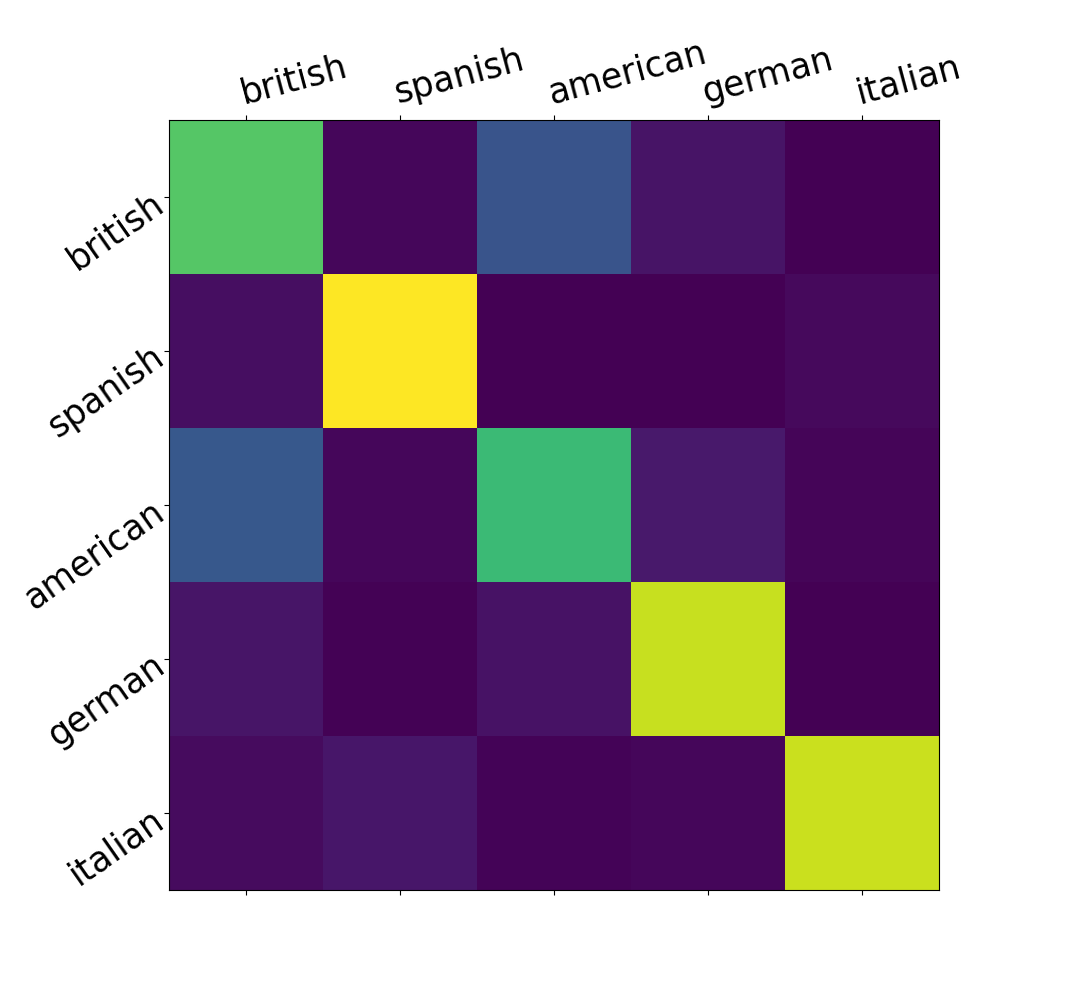
\includegraphics[width=\linewidth]{images/nec_confusion_matrix.png}
        \caption{confusion matrix representing the true positive distribution of the name-nationality dataset produced by a recurrent neural network}
        \label{fig:tp_scores}
\end{figure}

Another dataset that is a good showcase for the learnability imbalance is the CIFAR-10 [2] dataset (32$\times$32 RGB images of ten different classes) because it also contains similiar classes such as \emph{dog} and \emph{cat}.
%Another dataset that is a good showcase for the learnability imbalance is the CIFAR-10 [2] dataset because in the 10 different classes which consist of 32x32 pixel images, there are also similiar ones such as \emph{dog} and \emph{cat}.
When looking at the true positive rates produced by a convolutional neural network [3], trained on that dataset, it can be seen that there are some classes that got misclassified more often (in this case bird, cat, deer and dog) which hints to a more difficult learnability. 
The CIFAR-10 and the name-nationality dataset will be used for experiments in order to find methods for minimizing such variances in the evaluation scores.

\begin{figure}[h!]
        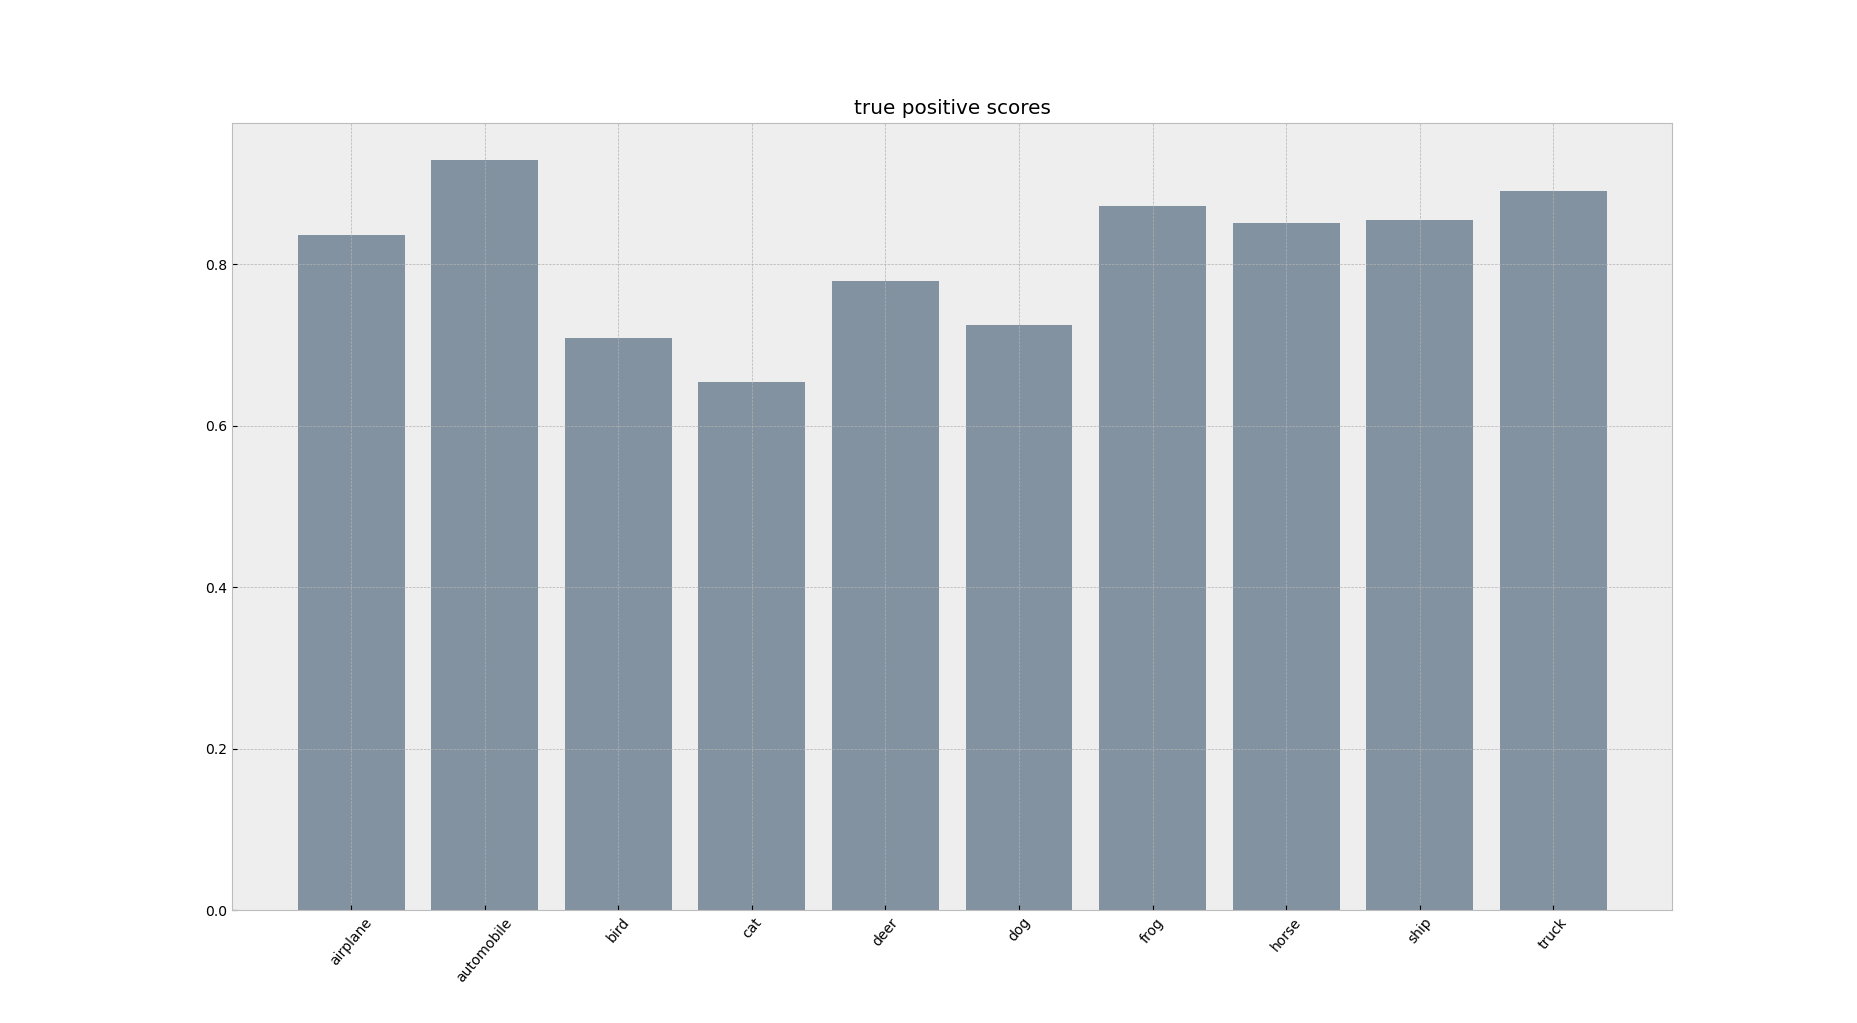
\includegraphics[width=\linewidth]{images/cifar10_tp_scores.png}
        \caption{true positive scores of a model trained on the CIFAR-10 dataset}
        \label{fig:tp2_scores}
\end{figure}

%---> When working with such datasets the learnability differences of the individual classes are mostly only identifiable after the model has been trained and evaluated normally.
%---> A confusion matrix or the calculation of the true positive rates then reveal what classes where learned the best and which should have received a higher weight. 

To figure out such methods one should first go back to the class imbalance problem because there are already solutions existing:
It is common to weight the error function [1] according to the size of each class, i.e. the number of samples it contains.
Therefore, for every class there is a weight, which is greater the fewer elements it contains and that gets multiplied with the loss produced by its samples. % "Therefore" wrong
%Since the aim of a neural network is to minimize the overall loss and samples from a smaller class will produce a higher error, they will have a higher impact on the learning process in order to compensate for the different class sizes.
That will cause, that samples from a smaller class will produce a higher error and, since the aim of a neural network is to minimize the loss [4], will have a higher impact of the learning process.
Another way to try to compensate for the different class sizes is to use more augmentation [5] on the samples of smaller classes. 
Augmentation describes the random transformation of the samples, in order to synthetically generate more input data for the model. For example, in image classification it is common to randomly flip, mirror or to add white noise to the images [6].
This can help the model generalizing better.
But since both methods rely on the different proportions of the classes in the dataset, the question arises how to apply them on datasets that, even though they don't suffer from class imbalance, still show a big learnability imbalance.
When working with such datasets the learnability differences of the individual classes are mostly only identifiable after the model has been trained and evaluated normally. 
A confusion matrix or the calculation of the true positive rates can then reveal what classes where learned the best and which should have received a higher weight. 
These rates can be used to determine which loss weights or how much data augmentation should be used for each class.


\begin{algorithm}[H]
        \caption{creating loss weights for a balanced dataset}

        \textit{\textbf{C} $\hat{=}$ amount of classes}
        \\
        %\\ \textit{\textbf{train(weights)} describes the initialization and the whole training process of a classification model using the loss-weights $weights$. \\$weights_i$ will be multiplied to every loss generated by a sample of class $i$.}
        \\ \textit{\textbf{train(weights)} describes the initialization and training process of a classification model in which $weights_i$ will be multiplied to every loss generated by a sample of class $i$.}
        \\
        \\ \textit{\textbf{evaluate()} creates the set $s$ with $\left|s\right|$ = $C$ and $s_i \in [0;1]$ which contains the true positive scores of all classes of the test dataset}
        \\
        \\ \textit{\textbf{W(s)} is a function that creates a set of loss-weights $w$ with $\left|w\right|$ = $C$ and $w_i \in [0;1]$ using a set of true positive scores $s$: $W: s \rightarrow w$ ; $\{s_i,...,s_C\} \rightarrow \{w_i,...,w_C\}$ }
        \\
        \\ \textit{\textbf{process:}}
        \begin{algorithmic}[1]
         \STATE $train(weights=\{w_1=1, w_2=1, ..., w_c=1\}$)
         \STATE $s = evaluate()$
         \STATE $w = W(s)$
         \STATE $train(weights=w)$
         \STATE $s_{new} = evaluate()$
         \STATE $compare(s, s_{new})$

        \end{algorithmic}
\end{algorithm}


%\begin{algorithm}[H]
%        \caption{creating loss weights for a balanced dataset}
%        \begin{algorithmic}[1]
%
%         \STATE D $:=$ dataset\\
%         \STATE L $:=$ loss(y, $\hat{y}$)\\
%         \STATE W $:=$ calculateWeights(scores)\\
%         \STATE classes $:=$ \{1, 2, ..., C ; C $\hat{=}$ amount of classes\}\\
%         %\STATE class := $C_i$
%         \textit{\textbf{forward}(x): describes the output of a neural network as a chained function with input x}\\
%         \textit{\textbf{backward}(y, $\hat{y}$): describes the backpropagation of the loss function w.r.t. the parameters of the neural network}
%         \textit{\textbf{evaluate}(): describes the calculation of the true positive rates of every class and returns a set with the length of C}\\
%
%        \\ \Procedure{train}{weights}
%         \FOR{\textbf{each} (sample, target, class) in D}\\
%                \STATE output := forward(sample)\\
%                \STATE error := weights$_{class} *$ L(output, target)\\
%                \STATE backward(error)\\
%         \ENDFOR\\
%         \EndProcedure\\
%         \STATE train(weights=$\{w_1=1, w_2=1, ..., w_C=1\}$)
%         \STATE truePositiveScores = evaluate()
%         \STATE lossWeights = W(truePositiveScores)
%         \STATE train(weights=lossWeights)
%
%
%        \end{algorithmic}
%\end{algorithm}


%
%
%The figure 1 below shows the true positive rates of a an evaluated convolutional neural network [2] that was trained on the CIFAR-10 dataset, which contains 32$\times$32 RGB images of ten different classes [3].
%This dataset is a good show case for the learnability imbalance problem since it contains similiar classes, such as \emph{dog} and \emph{cat} and will be used as one of the main datasets to run the research experiments on.
 
% Figure \ref{fig:tp_scores} shows true positive scores.

%Looking at the true positive rates it can be seen that there are some classes that got misclassified more often (in this case bird, cat deer and dog). 
%Since this dataset is mostly used to present experimental results and is, due to its small sample dimensions, a more simple classification task, 
%such a variance in the evaluations scores mostly doesn't matter. But when it comes to datasets that a model has to be trained on for a real world usecase 
%it is optimal to have a fair and unbiased class distribution. An example in natural language processing [4] is \emph{name-ethnicity classification} 
%where a model predicts the ethnicity of a name only by its letters [5]. Names from nationalities that speak the same language (e.g. british and american) result in a lower accuracy
%which therefore can lead to wrong interpretations when the model is used for social sciences experiments. The figure 2 shows a low accuracy for the \emph{british} class which comes
%especially from the presence of the similiar \emph{american} class.
%Therefore, additionally to the CIFAR-10 dataset, experiments on how to counteract learnability-imbalance will also be done on a name-nationality dataset using a recurrent neural network architecture [6].



\section{state of the art}
TODO first section here


\section{approach}
TODO second section here


\section{third section}
TODO third section here


\begin{thebibliography}{1}

\bibitem{}
Name Name, Name Name, Name Name (2006). Title, 24(1), 29-33.

\end{thebibliography}


\end{document}

% biased class distribution: https://link.springer.com/chapter/10.1007/3-540-44795-4_45#:~:text=Labeled%20data%20for%20classification%20could,optimal%20classification%20on%20new%20data.
% class imbalance over sampling: https://machinelearningmastery.com/random-oversampling-and-undersampling-for-imbalanced-classification/